\documentclass[11pt,letterpaper]{article}

\usepackage[utf8]{inputenc}
\usepackage[margin=0.9in]{geometry}
\usepackage{hyperref}
\usepackage{xcolor}
\usepackage{graphicx}
\usepackage{listings}
\usepackage{booktabs}
\usepackage{amsmath}
\usepackage{tikz}
\usepackage{fancyhdr}
\usepackage{titlesec}
\usepackage{enumitem}

\usetikzlibrary{shapes.geometric, arrows, positioning, fit, backgrounds}

% Define Colors
\definecolor{primaryblue}{RGB}{41, 128, 185}
\definecolor{darkslate}{RGB}{44, 62, 80}
\definecolor{codebg}{RGB}{245, 247, 250}
\definecolor{accentgreen}{RGB}{39, 174, 96}
\definecolor{accentred}{RGB}{231, 76, 60}

\setlength{\headheight}{14pt}

\hypersetup{
    colorlinks=true,
    linkcolor=primaryblue,
    filecolor=primaryblue,
    urlcolor=primaryblue,
    citecolor=primaryblue,
    pdftitle={Plush Toy SCADA and Telemetry System: SWE Intern Handbook},
    pdfauthor={EnigmaK9 and Pineapple Engineering}
}

% Header and Footer
\pagestyle{fancy}
\fancyhf{}
\rhead{\textcolor{darkslate}{\small \textbf{Plush Toy SCADA Platform} \textbar\ SWE Intern Handbook}}
\lhead{\textcolor{darkslate}{\small System Architecture \& Operations}}
\rfoot{\thepage}
\renewcommand{\headrulewidth}{0.4pt}
\renewcommand{\footrulewidth}{0.4pt}

% Section styling
\titleformat{\section}
  {\normalfont\Large\bfseries\color{darkslate}}{\thesection}{1em}{}[\titlerule]
\titleformat{\subsection}
  {\normalfont\large\bfseries\color{primaryblue}}{\thesubsection}{1em}{}

% Listings configuration
\lstset{
  backgroundcolor=\color{codebg},
  basicstyle=\ttfamily\footnotesize,
  breaklines=true,
  captionpos=b,
  commentstyle=\color{accentgreen},
  keywordstyle=\color{primaryblue}\bfseries,
  stringstyle=\color{accentred},
  frame=single,
  rulecolor=\color{lightgray},
  tabsize=2,
  showstringspaces=false
}

\begin{document}

\begin{titlepage}
    \centering
    \vspace*{1.5cm}
    
    {\Huge \textbf{\color{darkslate}Industrial SCADA \& Telemetry Systems}}\\[0.4cm]
    {\LARGE \textbf{\color{primaryblue}Software Engineer Intern \& Junior Developer Handbook}}\\[0.8cm]
    
    \rule{\textwidth}{1.5pt}\\[0.5cm]
    {\large \textbf{An End-to-End Practical Guide to Architecture, SQLite Relational Modeling, and Real-Time Dashboards for Plush Toy Manufacturing}}\\[0.5cm]
    \rule{\textwidth}{1.5pt}\\[2cm]

    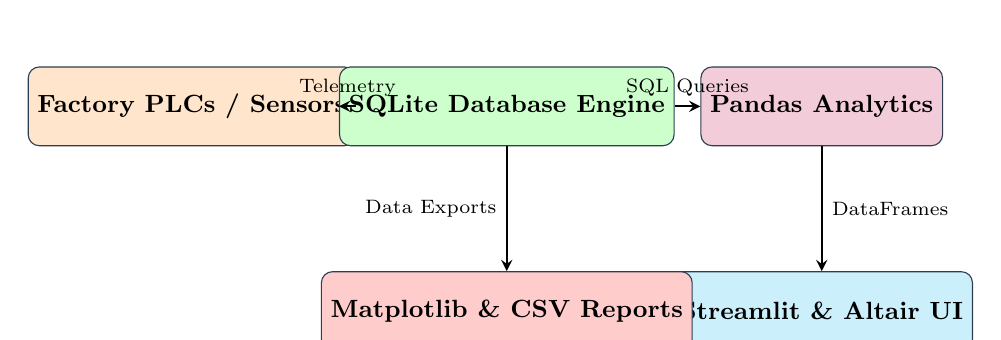
\begin{tikzpicture}[node distance=1.8cm, auto]
        \tikzstyle{box} = [rectangle, rounded corners, minimum width=2.8cm, minimum height=1cm, text centered, draw=darkslate, fill=blue!10, font=\bfseries\small]
        \tikzstyle{arrow} = [thick,->,>=stealth]

        \node (plc) [box, fill=orange!20] {Factory PLCs / Sensors};
        \node (sqlite) [box, fill=green!20, right of=plc, xshift=2.2cm] {SQLite Database Engine};
        \node (pandas) [box, fill=purple!20, right of=sqlite, xshift=2.2cm] {Pandas Analytics};
        \node (ui) [box, fill=cyan!20, below of=pandas, yshift=-0.8cm] {Streamlit \& Altair UI};
        \node (reports) [box, fill=red!20, below of=sqlite, yshift=-0.8cm] {Matplotlib \& CSV Reports};

        \draw [arrow] (plc) -- node[above] {\scriptsize Telemetry} (sqlite);
        \draw [arrow] (sqlite) -- node[above] {\scriptsize SQL Queries} (pandas);
        \draw [arrow] (pandas) -- node[right] {\scriptsize DataFrames} (ui);
        \draw [arrow] (sqlite) -- node[left] {\scriptsize Data Exports} (reports);
    \end{tikzpicture}

    \vfill
    
    \begin{minipage}{0.5\textwidth}
        \textbf{Author:} EnigmaK9 Engineering Team\\
        \textbf{Repository:} \texttt{israel-pineapple}\\
        \textbf{Target Audience:} Junior Software Engineers \& SWE Interns
    \end{minipage}
    \hfill
    \begin{minipage}{0.4\textwidth}
        \flushright
        \textbf{Version:} 1.0.0\\
        \textbf{Platform:} Linux / macOS / Windows\\
        \textbf{Language:} Python 3.10+
    \end{minipage}

\end{titlepage}

\newpage
\tableofcontents
\newpage

\section{Introduction: The Big Picture (What is SCADA?)}

Welcome to industrial software engineering! As a software engineer working on modern manufacturing systems, you bridge the gap between physical machinery and cloud/web applications.

\subsection{Physical Floor vs. Software Layer}
In a manufacturing plant:
\begin{itemize}[leftmargin=*]
    \item \textbf{Machines \& Stations:} Physical lines perform mechanical tasks (cutting fabric, stuffing plush bodies with synthetic fiber, stitching embroidered faces).
    \item \textbf{PLCs (Programmable Logic Controllers):} Small, rugged computers that read sensors (counting optical pulses as completed toys pass a laser, monitoring thermocouples on hot needles).
    \item \textbf{SCADA (Supervisory Control and Data Acquisition):} The supervisory system that gathers telemetry pulses, saves them to a database, calculates KPIs, and visualizes them on screens for operators and plant managers.
\end{itemize}

\subsection{Why This Project Matters}
Without a centralized telemetry platform, if Station 1 starts overheating and ruining teddy bears at 12:00 PM, nobody notices until hundreds of broken bears pile up in the trash bin. With our platform, the system flags a warning the second the scrap rate crosses 5\% or head temperature exceeds safe operating thresholds.

\section{System Architecture \& Component Diagram}

The repository \texttt{israel-pineapple} is organized into four clean layers following the \textbf{Separation of Concerns (SoC)} software design principle:

\begin{figure}[h!]
\centering
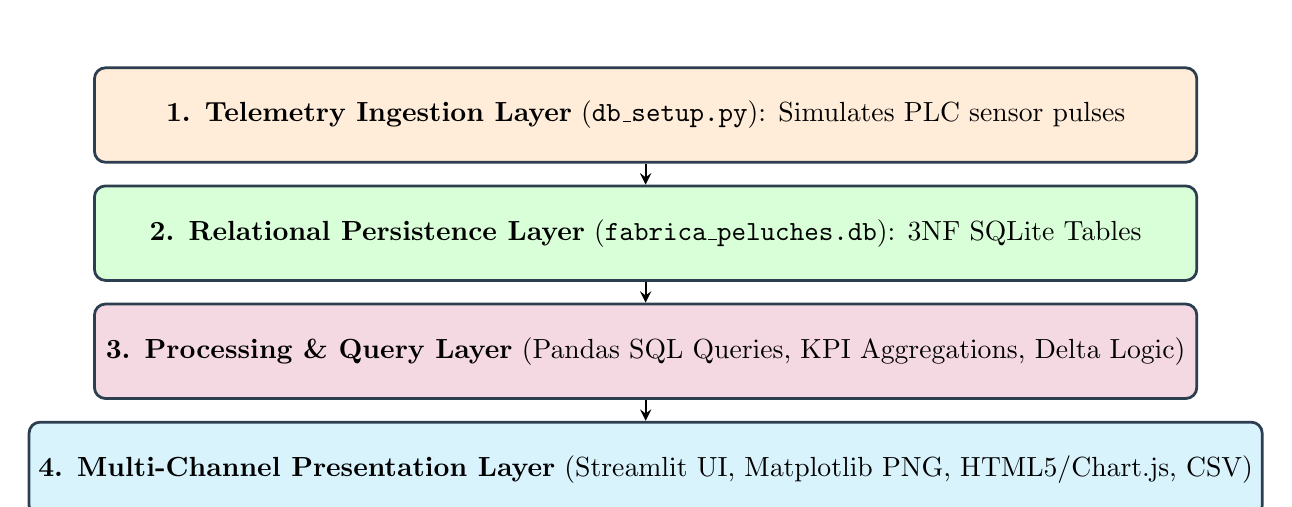
\begin{tikzpicture}[node distance=1.5cm]
    \tikzstyle{layer} = [rectangle, rounded corners, minimum width=14cm, minimum height=1.2cm, draw=darkslate, line width=1pt, text centered]
    
    \node (layer1) [layer, fill=orange!15] {\textbf{1. Telemetry Ingestion Layer} (\texttt{db\_setup.py}): Simulates PLC sensor pulses};
    \node (layer2) [layer, fill=green!15, below of=layer1] {\textbf{2. Relational Persistence Layer} (\texttt{fabrica\_peluches.db}): 3NF SQLite Tables};
    \node (layer3) [layer, fill=purple!15, below of=layer2] {\textbf{3. Processing \& Query Layer} (Pandas SQL Queries, KPI Aggregations, Delta Logic)};
    \node (layer4) [layer, fill=cyan!15, below of=layer3] {\textbf{4. Multi-Channel Presentation Layer} (Streamlit UI, Matplotlib PNG, HTML5/Chart.js, CSV)};

    \draw [thick, ->, >=stealth] (layer1) -- (layer2);
    \draw [thick, ->, >=stealth] (layer2) -- (layer3);
    \draw [thick, ->, >=stealth] (layer3) -- (layer4);
\end{tikzpicture}
\caption{Four-Layer Architecture of the SCADA Monitoring System.}
\end{figure}

\section{Database Engineering with SQLite}

Rather than storing unstructured data, we use a structured relational database with SQLite. It requires zero server setup and stores everything inside a single, fast local file.

\subsection{Database Schema}
The database \texttt{fabrica\_peluches.db} models the factory with two relational tables:

\begin{table}[h!]
\centering
\small
\begin{tabular}{llll}
\toprule
\textbf{Table} & \textbf{Column} & \textbf{Data Type} & \textbf{Description} \\
\midrule
\texttt{lineas} & \texttt{id\_linea} & INTEGER PRIMARY KEY & Unique line identifier \\
 & \texttt{nombre} & TEXT NOT NULL & Name of station (e.g., Sewing Line 1) \\
 & \texttt{modelo\_peluche} & TEXT NOT NULL & Product model (e.g., Classic Teddy Bear) \\
\midrule
\texttt{produccion\_scada} & \texttt{id} & INTEGER PRIMARY KEY & Auto-incrementing record ID \\
 & \texttt{id\_linea} & INTEGER (FK) & References \texttt{lineas(id\_linea)} \\
 & \texttt{fecha\_hora} & TEXT NOT NULL & Shift hour (e.g., \texttt{08:00}, \texttt{09:00}) \\
 & \texttt{piezas\_buenas} & INTEGER NOT NULL & Count of approved toys produced \\
 & \texttt{piezas\_defectuosas} & INTEGER NOT NULL & Count of defective scrap toys \\
 & \texttt{temperatura\_maquina} & REAL NOT NULL & Tool head temperature in Celsius ($^\circ\text{C}$) \\
\bottomrule
\end{tabular}
\caption{Database Schema Definition.}
\end{table}

\subsection{Industrial KPI Mathematical Formulas}
When pulling data from SQLite into Python using Pandas, the business logic evaluates key production indicators:
\begin{equation}
\text{Total Good Units} = \sum_{i=1}^{n} \text{piezas\_buenas}_i
\end{equation}
\begin{equation}
\text{Total Scrap Units} = \sum_{i=1}^{n} \text{piezas\_defectuosas}_i
\end{equation}
\begin{equation}
\text{Scrap Rate (\%)} = \left( \frac{\text{Total Scrap}}{\text{Total Good} + \text{Total Scrap}} \right) \times 100
\end{equation}
\begin{equation}
\text{Average Temperature} = \frac{1}{n} \sum_{i=1}^{n} \text{temperatura\_maquina}_i
\end{equation}

\section{Code Walkthrough: File by File}

\subsection{\texttt{db\_setup.py} (Database Initializer \& Telemetry Simulator)}
This script builds the database schema and generates historical shift records. It purposefully creates an equipment malfunction in Line 1 at 12:00 to verify alert triggers:
\begin{lstlisting}[language=Python]
# Deliberate machine anomaly simulation
if hora_str == "12:00":
    buenas = 25
    malas = 10     # Scrap spike!
    temp = 85.5    # Overheating needle!
\end{lstlisting}

\subsection{\texttt{app\_dashboard.py} (Streamlit Real-Time Dashboard)}
This is the core interactive web app. Key features:
\begin{enumerate}
    \item \textbf{Dynamic Line Filtering:} The sidebar lets the operator pick a production line. Under the hood, it executes a parameterized SQL query:
\begin{lstlisting}[language=SQL]
SELECT p.fecha_hora, p.piezas_buenas, p.piezas_defectuosas, 
       p.temperatura_maquina, l.nombre, l.modelo_peluche
FROM produccion_scada p
JOIN lineas l ON p.id_linea = l.id_linea
WHERE p.id_linea = ? ORDER BY p.id ASC;
\end{lstlisting}
    \item \textbf{Live SCADA Pulse Button:} Clicking the sidebar button executes an instant SQL \texttt{INSERT} and re-renders all Altair charts on the fly.
\end{enumerate}

\subsection{\texttt{dashboard\_peluches.py} (Matplotlib Shift Reporter)}
A batch utility designed for cron jobs or automated email attachments. It connects to SQLite, renders a dual-axis trend graph with custom styling, and saves \texttt{dashboard\_peluches.png}.

\subsection{\texttt{dashboard\_web.html} (Zero-Dependency Web Client)}
A self-contained HTML5 file utilizing \textbf{Chart.js} via CDN. It demonstrates how factory displays on the shop floor can render telemetry charts without requiring a Python environment.

\subsection{\texttt{generar\_csv.py} (ERP / Spreadsheet Exporter)}
Exports hourly operational metrics into \texttt{scada\_peluches.csv} formatted with embedded spreadsheet formulas for automated defect percentage calculations.

\section{Practical Execution: Step-by-Step Guide}

\begin{enumerate}[leftmargin=*]
    \item \textbf{Clone the Repository:}
    \begin{lstlisting}[language=bash]
git clone https://github.com/EnigmaK9/israel-pineapple.git
cd israel-pineapple
    \end{lstlisting}

    \item \textbf{Initialize Virtual Environment:}
    \begin{lstlisting}[language=bash]
python3 -m venv .venv
source .venv/bin/activate
    \end{lstlisting}

    \item \textbf{Install Dependencies:}
    \begin{lstlisting}[language=bash]
pip install -r requirements.txt
    \end{lstlisting}

    \item \textbf{Seed Database:}
    \begin{lstlisting}[language=bash]
python db_setup.py
    \end{lstlisting}

    \item \textbf{Launch Interactive Dashboard:}
    \begin{lstlisting}[language=bash]
streamlit run app_dashboard.py
    \end{lstlisting}
\end{enumerate}

\section{SWE Intern Field Rules \& Best Practices}

\begin{itemize}[leftmargin=*]
    \item \textbf{Never Use String Formatting for SQL:} Always use parameterized tuples \texttt{(param,)} to prevent SQL injection.
    \item \textbf{Handle Division by Zero:} If a newly commissioned machine has produced 0 units, $(0+0)=0$. Always check \texttt{if total > 0} before computing ratios.
    \item \textbf{Idempotent Scripts:} Database setup scripts must be safe to run multiple times without corrupting state or crashing on duplicate keys.
    \item \textbf{Commit Semantics:} Use descriptive conventional commit messages (\texttt{feat:}, \texttt{fix:}, \texttt{docs:}) to maintain a clean git history.
\end{itemize}

\end{document}
